\chapter{Detailed Calculation of the Quark Self Energy}\label{chap:appendixA}
This first appendix is denoted to the technical details of the conducted calculations. In order to obtain the final expression  for the quark self energy diagram $\Sigma_q(p)$, we need to perform three different integrations, i.\,e. the ususal integration over the loop momentum $q$, the Feynman parameter $x$, introduced to facilitate the momentum integration, and finally the integration over the spectral parameters $\lambda_1$ and $\lambda_2$, respectively. We will highlight the most important steps of each part of the calculation and present the full analytical expressions in the end.\\
The Feynman rules for QCD in the Landau gauge can be derived from \eqref{eqn:S_QCD}, they are summarized for example in the appendix of \cite{NPgaugeLecture}. 


\section*{General Tensor Structure and Manipulations}
 The relevant diagram for our computation of the quark spectral function is the one-loop contribution to the Dyson-Schwinger equation for the (inverse) quark propagator:
\begin{align}
\bigg(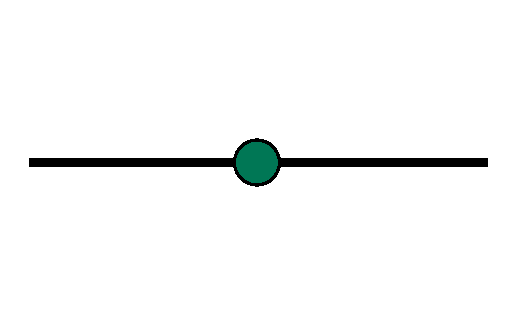
\includegraphics[scale=0.4, valign=c]{figs/diagrams/quarkDSE/full_quark_propagator}\bigg)^{-1} = 
\bigg(
\includegraphics[scale=0.4, valign=c]{figs/diagrams/quarkDSE/bare_quark_propagator.pdf}\bigg)^{-1} - 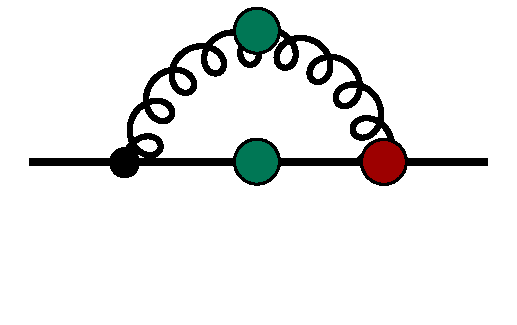
\includegraphics[scale=0.4, valign=c]{figs/diagrams/quarkDSE/quark_self_energy}
\end{align}
 Applying the Feynman rules for QCD in the Landau gauge  we find\footnote{Note, that we work in a classical vertex approximation, i.\,e. $\Gamma^{(3)}_{q\bar{q}A} \equiv S^{(3)}_{q\bar{q}A}$, as discussed in the main part. This explains the replacement of the red blob in this explicit visualization.}:
\begin{align*}
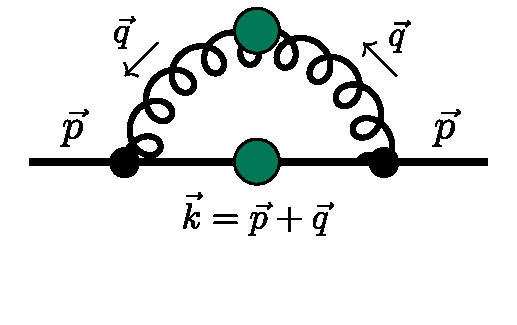
\includegraphics[scale=0.45, valign=c, trim = 0 6em 0 0]{figs/diagrams/quark_self_energy_classical} := \Sigma_q
(p) &= (-ig)^2 \delta^{ab}C_f \int_q\ \Pi^{\mu\nu}_{\perp}(q) G_A(q)\gamma_{\mu}G_q(p+q)\gamma_{\nu},
\end{align*}
with the transverse projection operator $\Pi^{\mu\nu}_{\perp}(q)$ as defined in (\ref{eqn:transversal_projector}). \\

For the gluon and quark propagators, we insert the respective  K\"all\'{e}n-Lehmann spectral representations, i.\,e.
\begin{align} 
G_A(q)&=\int_{\lambda_1} \frac{\lambda_1\rho_A(\lambda_1)}{q^{2}+\lambda_1^{2}},
\end{align}
and
\begin{equation}
\begin{aligned}
G_q(p+q) = \left(\slashed{p} + \slashed{q}\right) \int_{\lambda_2} \frac{\lambda_2\rho_{q}^D(\lambda_2)}{(p+q)^{2}+\lambda_2^2}+\int_{\lambda_2} \frac{\lambda_2\rho_q^M(\lambda_2)}{(p+q)^{2}+\lambda_2^2}.
\end{aligned}
\end{equation}
For a detailed discussion of the Dirac structure of the quark propagator we refer to \appref{chap:appendixB}. \\
The structure of the quark propagator allows us split the computation of the full diagram into two components, its Dirac vector and scalar part, i.\,e.
\begin{equation}
	\Sigma_q(p) =\slashed{p}\cdot\Sigma_{q}^D(p) + \Sigma_{q}^M(p).
\end{equation}
Whereas the scalar part $\Sigma_{q}^M(p)$ does not contain any additional gamma matrices, we have to be very careful when permuting the tensor structure of the vector part $\Sigma_{q}^M(p)$, where an additional gamma matrix is inherently implemented via $\slashed{p}= p^{\alpha}\gamma_{\alpha}$. To be able to contract the Dirac indices of the transversal propagator with the two uncontracted indices of the vertices, we need to take care of the following, well known identities, cf. \cite{PeskinSchroeder1995}:
\begin{align}
\left\{\gamma_{\alpha},\gamma^{\nu}\right\} &= 2\delta_{\alpha}^{\phantom{{\alpha}}\nu}, \\
\gamma_{\mu}\gamma^{\mu} &= d, \\
\slashed{p}^2 &= p^2.
\end{align}
After carefully permuting all relevant terms we are left with:
\begin{equation}
	\begin{aligned}
		\slashed{p}\cdot\Sigma_{q}^D(p) &\sim \int_q \left((3-d)\slashed{p} + \left(\color{MScRed}(1-d)\normalcolor - \color{MScGreen}2\ \frac{p\cdot q}{q^2}\normalcolor\right)\slashed{q}\right)\int\limits_{\left\{\lambda_1,\lambda_2\right\}} \frac{\lambda_1\rho_A(\lambda_1)}{q^2 + \lambda_1^2} \frac{\lambda_2\rho_q^D(\lambda_2)}{(p+q)^2 + \lambda_2^2}, \\[0.5em]
		\Sigma_{q}^M(p) &\sim \int_q\ (d-1)\int\limits_{\left\{\lambda_1,\lambda_2\right\}} \frac{\lambda_1\rho_A(\lambda_1)}{q^2 + \lambda_1^2} \frac{\lambda_2\rho_q^M(\lambda_2)}{(p+q)^2 + \lambda_2^2}.
	\end{aligned}
\end{equation}
The nontrivial contributions arising from above considerations are highlighted in red and green. In the following we will manipulate all terms individually from left to right. Note, that the first (uncolored) term of the vector part has the same momentum structure as the scalar part, up to prefactors. \\
In a first step the integration order $q\leftrightarrow\left\{\lambda_1,\lambda_2\right\}$ is swapped, which is only allowed for finite integrands, according to Fubinis theorem. We already explained how to resolve this issue in the main part of this work, for an overview cf. \figref{fig:spectral_renormalization}. \\ Introducing Feynman parameters according to 
\begin{equation}
\frac{1}{A B}=\int_{0}^{1} \dd x\ \frac{1}{x A+(1-x) B},
\end{equation}
allows us to recast the first term as follows:
\begin{equation}
	(3-d)\slashed{p} \int_q \frac{1}{q^2 + \lambda_1^2}\frac{1}{(p+q)^2 + \lambda_2^2} = (3-d)\slashed{p}\int_{x,q} \frac{1}{\left[q^2 + \Delta_1\right]^2},
\end{equation}
where we defined
\begin{equation}
	\Delta_1 = x(1-x)p^2 + (1-x)\lambda_1^2 + x\lambda_2^2,
\end{equation}
and shifted the loop momentum $q \rightarrow q-xp$. As observed above, the same holds for the Dirac scalar part $\Sigma_{q}^M(p)$, the only difference is the prefactor of $(d-1)$. \\
 The term highlighted in red is a bit trickier since it involves another factor of $q^{\alpha}$ that is affected by the shift of the loop momentum: 
\begin{equation}
\begin{aligned}
	(1-d)\gamma_{\alpha} \int_q q^{\alpha} \frac{1}{q^2 + \lambda_1^2}\frac{1}{(p+q)^2 + \lambda_2^2} &= (1-d)\gamma_{\alpha}\int_{x,q} (q^{\alpha} - xp^{\alpha})\frac{1}{\left[q^2 + \Delta_1\right]^2}\\
	&= (d-1)\slashed{p}\int_{x,q}\frac{x}{\left[q^2 + \Delta_1\right]^2}.
	\end{aligned}
\end{equation}
In the last line we used the fact, that all integrations involving an odd power of $q$ in the numerator are zero.\\
 Following the same line of arguments, we can also simplify the third relevant term, highlighted in green. It features additional factors of $p$ and $q$ and an additional contribution to the denominator:
\begin{equation}
	\begin{aligned}
		-2\gamma_{\alpha} \int_q q^{\alpha}\frac{p\cdot q}{q^2} \frac{1}{q^2 + \lambda_1^2}\frac{1}{(p+q)^2 + \lambda_2^2} = -2\frac{\gamma_{\alpha}p_{\beta}}{\lambda_1^2}\int_q\left\{\left(\frac{ q^{\alpha}q^{\beta}}{q^2 ((p+q)^2 + \lambda_2^2)}\right)\right.\\ \left. - \left(\frac{ q^{\alpha}q^{\beta}}{(q^2 + \lambda_1^2)((p+q)^2 + \lambda_2^2)}\right)\right\}.
	\end{aligned}
\end{equation}
We decomposed the first part of the integrand using partial fraction decomposition,
\begin{equation}
\frac{1}{q^{2}} \frac{1}{q^{2}+\lambda_1^{2}}=\frac{1}{\lambda_1^{2}}\left(\frac{1}{q^{2}}-\frac{1}{q^{2}+\lambda_1^{2}}\right),
\end{equation}
in order to reduce the complexity of the denominator. Now we can again perform the Feynman trick and shift the loop momentum $q\rightarrow q-xp$ to obtain
\begin{equation}
	\cdots = -2\frac{\gamma_{\alpha}}{\lambda_1^2}\int_{x,q}\left\{ \left((p\cdot q)q^{\alpha} + x^2p^2p^{\alpha}\right)\left(\frac{1}{\left[q^2 + \Delta_2\right]^2} - \frac{1}{\left[q^2 + \Delta_1\right]^2}\right) \right\},
\end{equation}
where we again discarded all terms that were odd in $q$. Additionally we define
\begin{equation}
	\Delta_2 = \Delta_1 - (1-x)\lambda_1.
\end{equation}
In the first part of this expression we symmetrize the momenta according to 
\begin{equation}
	q^{\alpha}q^{\beta} = \frac{1}{d}\delta^{\alpha\beta}q^2,
\end{equation}
which is valid under the integral, and therefore find in total:
\begin{equation}
	\cdots = -2\frac{\slashed{p}}{\lambda_1^2}\int_{x,q}\left\{\frac{1}{d}\left(\frac{q^2}{\left[q^2 + \Delta_2\right]^2} - \frac{q^2}{\left[q^2 + \Delta_1\right]^2}\right) + p^2x^2\left(\frac{1}{\left[q^2 + \Delta_2\right]^2} - \frac{1}{\left[q^2 + \Delta_1\right]^2}\right)\right\}
\end{equation}
To condense our notation, we sort the contributions to both parts of the diagram in  powers of $q^2$ and collect the prefactors as coefficients $A_i$, $B_i$ and $C_i$. This concludes the first part of the calculation and renders the loop momentum integration trivial. We arrive at
\begin{align}
\Sigma_{q}^D(p) &= (-ig)^2\delta^{ab}C_f\int\limits_{\left\{\lambda_1,\lambda_2\right\}}\lambda_1\lambda_2\rho_A(\lambda_1)\rho_q^D(\lambda_2)\cdot I_q^D\left(p, \lambda_1, \lambda_2,x\right),\\
\Sigma_{q}^M(p) &= (-ig)^2\delta^{ab}C_f\int\limits_{\left\{\lambda_1,\lambda_2\right\}}\lambda_1\lambda_2\rho_A(\lambda_1)\rho_q^M(\lambda_2)\cdot I_q^M\left(p, \lambda_1, \lambda_2,x\right),
\end{align}

with the respective integrands defined as
\begin{align}
I_q^D\left(p, \lambda_1, \lambda_2,x\right)&=\int_{q, x} \sum_{i=0}^{1}\left(q^{2}\right)^{i}\left[\frac{A_{i}}{\left[q^{2}+\Delta_{1}\right]^{2}}-\frac{B_{i}}{\left[q^{2}+\Delta_{2}\right]^{2}}\right],\\
I_q^M\left(p, \lambda_1, \lambda_2,x\right)&=\int_{q, x} \sum_{i=0}^{1}\left(q^{2}\right)^{i}\left[\frac{C_{i}}{\left[q^{2}+\Delta_{1}\right]^{2}}\right],
\end{align}
and the  coefficients are given by
\begin{equation}
\begin{alignedat}{3}
&A_0 = \frac{2p^2x^2}{\lambda_1^2}+ 3x -1,   \qquad  &&B_0 = \frac{2p^2x^2}{\lambda_1^2},    \qquad       &&C_0 = 3, \\
&A_1 = \frac{1}{2\lambda_1^2},  			 \qquad  &&B_1 = \frac{1}{2\lambda_1^2},          \qquad  	  &&C_1 = 0. \\
\end{alignedat}
\end{equation}
Note, that the presented coefficients are already evaluated in $d=4$, we explicitly checked, that they do not change when going to $d=4-2\varepsilon$ and performing the limit $\varepsilon\rightarrow 0$, which will be discussed in more detail in the subsequent section.

\section*{Loop Momentum Integration}
In this form, the momentum integration can be performed using standard integration formulae known in the context of dimensional regularization, the regularization scheme of our choice. The respective integrals are solved via
\begin{equation}
	\int\frac{\dd^d q}{(2\pi)^d}\frac{(q^2)^m}{\left[q^2 + \Delta\right]^n} = \frac{1}{(4\pi)^{d/2}}\frac{\Gamma(m+\frac{d}{2})\Gamma(n-\frac{d}{2}-m)}{\Gamma(\frac{d}{2})\Gamma(n)} \Delta^{m+d/2-m},
\end{equation} 
with $m$ a non-negative and $n$ a positive integer \cite{PeskinSchroeder1995}. For our computation the relevant expressions have $n=2$ and $m= 0,1$. Explicitly, the term with $m=0$ evaluates to
\begin{equation}
\begin{aligned}
	\int \frac{\dd^d q}{(2\pi)^d} \frac{1}{\left[q^2 + \Delta\right]^2} &\overset{\phantom{(*)}}{=}  \frac{1}{(4\pi)^{\frac{d}{2}}} \frac{\Gamma(2-\frac{d}{2})}{\Gamma(2)} \Delta^{\frac{d}{2}-2} \\
	&\overset{(*)}{=} \frac{1}{(4\pi)^{2}}\left(\frac{1}{\varepsilon} - \operatorname{log}\Delta - \gamma_{\mathrm{E}} + \operatorname{log} 4\pi + \operatorname{log} \mu^2 + \mathcal{O}(\varepsilon)\right)\\
	&\overset{\phantom{(*)}}{=} \frac{1}{(4\pi)^{2}}\left(\frac{1}{\varepsilon} - \operatorname{log}\Delta + \operatorname{log}\left(\frac{4\pi\mu^2}{\operatorname{e}^{\gamma_{\mathrm{E}}}}\right)   + \mathcal{O}(\varepsilon)\right),
	\end{aligned}
\end{equation}
where we evaluate for $d= 4 -2\varepsilon$ and expand the relevant quantities up to lowest order in the limit $\varepsilon\rightarrow 0$. Note, that to account for this change in the dimensionality, we introduced a factor of $\mu^{2\varepsilon}$ under the integral. Here, $\Gamma(n)$ is the usual gamma function and  $\gamma_{\mathrm{E}}\approx 0.57722$ is the Euler-Mascheroni constant.\\ This isolates the divergence of the diagram in the $\frac{1}{\varepsilon}$-term, which is discarded, as usual. Note, that as a remnant of swapping the integration order we are not done yet and still need to renormalize the spectral integrands appropriately. The second important integral ($n=2$ and $m=1$) is solved analogously:
\begin{equation}
\begin{aligned}
	\int \frac{\dd^d q}{(2\pi)^d} \frac{q^2}{\left[q^2 + \Delta\right]^2} &=  \frac{1}{(4\pi)^{\frac{d}{2}}} \frac{\Gamma(1+\frac{d}{2})\Gamma(1-\frac{d}{2})}{\Gamma(\frac{d}{2})\Gamma(2)} \Delta^{\frac{d}{2}-1} \\
	&= \frac{1}{(4\pi)^{\frac{d}{2}}}\left(\frac{d}{2-d}\right)\Gamma\big(2-\frac{d}{2}\big) \Delta\cdot\Delta^{\frac{d}{2}-2} \\
	&= \frac{-2}{(4\pi)^{2}}\Delta\left(\frac{1}{\varepsilon} +\frac{1}{2}- \operatorname{log}\Delta - \gamma_{\mathrm{E}} + \operatorname{log} 4\pi + \operatorname{log} \mu^2 + \mathcal{O}(\varepsilon)\right)\\
	&= \frac{-2}{(4\pi)^{2}}\Delta\left(\frac{1}{\varepsilon} +\frac{1}{2} - \operatorname{log}\Delta + \operatorname{log}\left(\frac{4\pi\mu^2}{\operatorname{e}^{\gamma_{\mathrm{E}}}}\right)   + \mathcal{O}(\varepsilon)\right),
	\end{aligned}
\end{equation}
where we used the properties of the gamma function, $\Gamma(z+1)=z\Gamma(z)\ \forall z\in \mathbb{C}$.\\

Reordering the expression in powers of the Feynman parameter $x$, we arrive at:
\begin{align}
I_q^D\left(p, \lambda_1, \lambda_2\right) &=\left(\frac{1}{\varepsilon}+\log \left(\frac{4 \pi \mu^{2}}{e^{\gamma_{\mathrm{E}}}}\right)\right) \sum\limits_{i=0}^{2}\left( \frac{\alpha_{i}-\beta_{i}}{i+1}\right) - \frac{1}{4}\nonumber\\
&-\mathlarger{\int}_{x} \sum\limits_{i=0}^{2} x^{i}\left(\alpha_{i} \log \Delta_{1}-\beta_{i} \log \Delta_{2}\right)   + \mathcal{O}(\varepsilon) \label{eqn:IqD}\\[0.5em]
I_q^M\left(p, \lambda_1, \lambda_2\right)&=\left(\frac{1}{\varepsilon}+\log \frac{4 \pi \mu^{2}}{e^{\gamma_{\mathrm{E}}}}\right) \gamma_0
-\mathlarger{\int}_{x} \gamma_{0} \log \Delta_{1} +\mathcal{O}(\varepsilon).\label{eqn:IqM}
\end{align}


We will present the full analytical expressions for the coefficients and integrals on the next pages. Note, that the prefactor of $1/(4\pi)^2$ is pulled out of the integrand in order to replace $\alpha = g^2/(4\pi)$ in the global prefactor.

\section*{Feynman Parameter Integration}
In the next step, the respective Feynman integrals can be performed. We use standard Mathematica integration routines and compare the results of the explicit integrations with  numerical integration as a benchmark check. The relevant integrals are  
\begin{align}
	f_i(p,\lambda_1, \lambda) &\sim \int_0^1 \dd x\ x^{i} \operatorname{log}\Delta_1 \\
g_i(p,\lambda_1, \lambda) &\sim \int_0^1 \dd x\ x^{i} \operatorname{log}\Delta_2 \\
h_0(p,\lambda_1, \lambda) &= \int_0^1 \dd x\ \operatorname{log}\Delta_1
\end{align}
with $i$ ranging from 0 to 2. The lengthy expressions are displayed on the next pages, together wit the reordered coefficients introduced above.\\ This completes the first major part of the calculation, we now need to focus on the renormalization of the the obtained expressions in order to access the final result for the spectral integrands, that serve as an input to our iterative procedure. 

\afterpage{%
\newgeometry{width=180mm,top=3cm}
\begin{landscape}
	\begin{center}
		\newcommand{\col}[1]{\label{eq:coeff_A_#1}\qquad\qquad}
\newenvironment{titledeqns}[1]{\large\bfseries{#1}
}{}

\newcommand{\tunedvs}{3pt}

\makeatletter 
\def\leqno{\tagsleft@true}\def\reqno{\tagsleft@false} 
\makeatother 

\leqno

\hspace{0pt}
%\vspace{1em}
\begin{titledeqns}{Coefficients and Explicit Expressions for the Feynman Parameter Integration - Dirac Vector Part I}
%\vfill
\begin{align}
 \alpha_0 &= -2, \\[1em]
\alpha_1 &= -\frac{p^2+\lambda_2^2 - 4\lambda_1^2}{\lambda_1^2}, \\[1em]
\alpha_2 &= \frac{3p^2}{\lambda_1^2}, \\[3em]
f_0 &= \frac{1}{p^2}\left[\left(\lambda_1^2-\lambda_2^2\right)  \operatorname{log} \left(\frac{\lambda_2}{\lambda_1}\right)+\zeta\cdot \operatorname{arcoth}\left(\frac{\lambda_2^2+\lambda_1^2+p^2}{\zeta}\right)\right] + \operatorname{log} (\lambda_2)+ \operatorname{log} (\lambda_1)-2, \\[1em]
f_1 &=  \frac{1}{4 p^4}\left[-\mathcal{D}_{\mathrm{cut}}\cdot\zeta\left(\lambda_2^2-\lambda_1^2+p^2\right) -2 p^2 \left(\lambda_2^2-\lambda_1^2+2 p^2\right)+2 \operatorname{log} (\lambda_2) \left(-\left(\lambda_2^2-\lambda_1^2\right)^2-2 \lambda_2^2 p^2+p^4\right)  \right. \\ &\hspace{3.81em}+2 \left. \operatorname{log} (\lambda_1) \left(-2 \lambda_2^2 \lambda_1^2+\lambda_1^4+\left(\lambda_2^2+p^2\right)^2\right)\right],\notag \\[1em]
 f_2 &= \frac{1}{18 p^6}\left[-\mathcal{D}_{\mathrm{cut}}\cdot 3\zeta \left(\lambda_1^4-\lambda_1^2 \left(2 \lambda_2^2+p^2\right)+\left(\lambda_2^2+p^2\right)^2\right) -p^2 \left(6 \left(\lambda_2^2-\lambda_1^2\right)^2+3 p^2 \left(5 \lambda_2^2-\lambda_1^2\right)+13 p^4\right)  \right. \\ &\hspace{3.81em}+6 \left.\operatorname{log} (\lambda_2) \left(-\left(\lambda_2^2-\lambda_1^2\right)^3+3 \lambda_2^2 p^2 \left(\lambda_1^2-\lambda_2^2\right)-3 \lambda_2^2 p^4+p^6\right)  \right.\notag \\ &\hspace{3.81em}+6 \left. \operatorname{log} (\lambda_1) \left(\lambda_2^2-\lambda_1^2+p^2\right) \left(\lambda_1^4+\lambda_1^2 \left(p^2-2 \lambda_2^2\right)+\left(\lambda_2^2+p^2\right)^2\right)\right], \notag
\end{align}
\end{titledeqns}
%\vfill

		\end{center}
\vspace{-2em}
where we defined
		\begin{align*}
\mathcal{D}_{\mathrm{cut}} = \operatorname{log} \left(\zeta - \lambda_1^2+\lambda_2^2-p^2\right)-\operatorname{log} \left(\zeta -\lambda_1^2 +\lambda_2^2+p^2\right)+\operatorname{log} \left(\zeta +\lambda_1^2-\lambda_2^2-p^2\right)-\operatorname{log} \left(\zeta +\lambda_1^2 -\lambda ^2+p^2\right),
\end{align*}	
with
\begin{equation*}
	\zeta=\sqrt{\lambda_1^{4}+\left(\lambda_2^{2}+p^{2}\right)^{2}+2 \lambda_1^{2}\left(p^{2}-\lambda_2^{2}\right)}.
\end{equation*}	

\begin{center}
		\pagebreak

\newcommand{\col}[1]{\label{eq:coeff_A_#1}\qquad\qquad}
\newenvironment{titledeqns}[1]{\large\bfseries{#1}
}{}

\newcommand{\tunedvs}{3pt}

\makeatletter 
\def\leqno{\tagsleft@true}\def\reqno{\tagsleft@false} 
\makeatother 

\leqno

\hspace{0pt}
\vspace{2em}
\begin{titledeqns}{Coefficients and Explicit Expressions for the Feynman Parameter Integration - Dirac Vector Part II}
\begin{align}
 \beta_0 &= 0,  \\[1em]
 \beta_1 &= -\frac{p^2+\lambda_2^2}{\lambda_1^2}, \\[1em]
 \beta_2 &= \frac{2p^2}{\lambda_1^2}, \\[3em]
 g_0 &= \frac{\lambda_2^2 \operatorname{log}\left(\frac{p^2}{\lambda_2^2}+1\right)}{p^2}+ \operatorname{log}\left(\lambda_2^2+p^2\right)-2, \\[1em]
 g_1 &=\frac{\left(\lambda_2^2+p^2\right)^2  \operatorname{log} \left(\lambda_2^2+p^2\right)-\left(\lambda_2^2+2 p^2\right) \left(2 \lambda_2^2  \operatorname{log} (\lambda_2)+p^2\right)}{2 p^4},\\[1em]
 g_2 &= -\frac{15 \lambda_2^2 p^4+6 \lambda_2^4 p^2+12  \operatorname{log} (\lambda_2) \left(\lambda_2^6+3 \lambda_2^4 p^2+3 \lambda_2^2 p^4\right)-6 \left(\lambda_2^2+p^2\right)^3  \operatorname{log} \left(\lambda_2^2+p^2\right)+13 p^6}{18 p^6}. \end{align}
\vspace{2em}
\end{titledeqns}

\begin{titledeqns}{Coefficients and Explicit Expressions for the Feynman Parameter Integration - Dirac Scalar Part}
\begin{align}
 \gamma_0 &= 3, \\[1em]
 h_0 &= f_0 = \frac{1}{p^2}\left[\left(\lambda_1^2-\lambda_2^2\right)  \operatorname{log} \left(\frac{\lambda_2}{\lambda_1}\right)+\zeta\cdot \operatorname{arcoth}\left(\frac{\lambda_2^2+\lambda_1^2+p^2}{\zeta}\right)\right] + \operatorname{log} (\lambda_2)+ \operatorname{log} (\lambda_1)-2. 
\end{align}
\end{titledeqns}

\reqno
		\end{center}	
\end{landscape}
\clearpage
\restoregeometry
}
\newpage
\section*{Renormalization of the Spectral Integrands}
The renormalization of the spectral integrands according to a BPHZ-scheme has already been discussed in great detail in the main part of this work. The general idea is to cancel the quadratic and logarithmic divergencies of the different parts of the diagram by subtraction of a Taylor expansion in all momenta about the renormalisation scale $\mu$, resulting in finite integrands in the limit $\varepsilon\rightarrow 0$.
Here, we just want to show some exemplary plots to visualize the effects of the subtraction procedure on different parts of the Dirac vector integrand $I_q^D(p)$.
 \begin{figure}[H] 
 \centering
	\begin{minipage}{0.8\textwidth}
		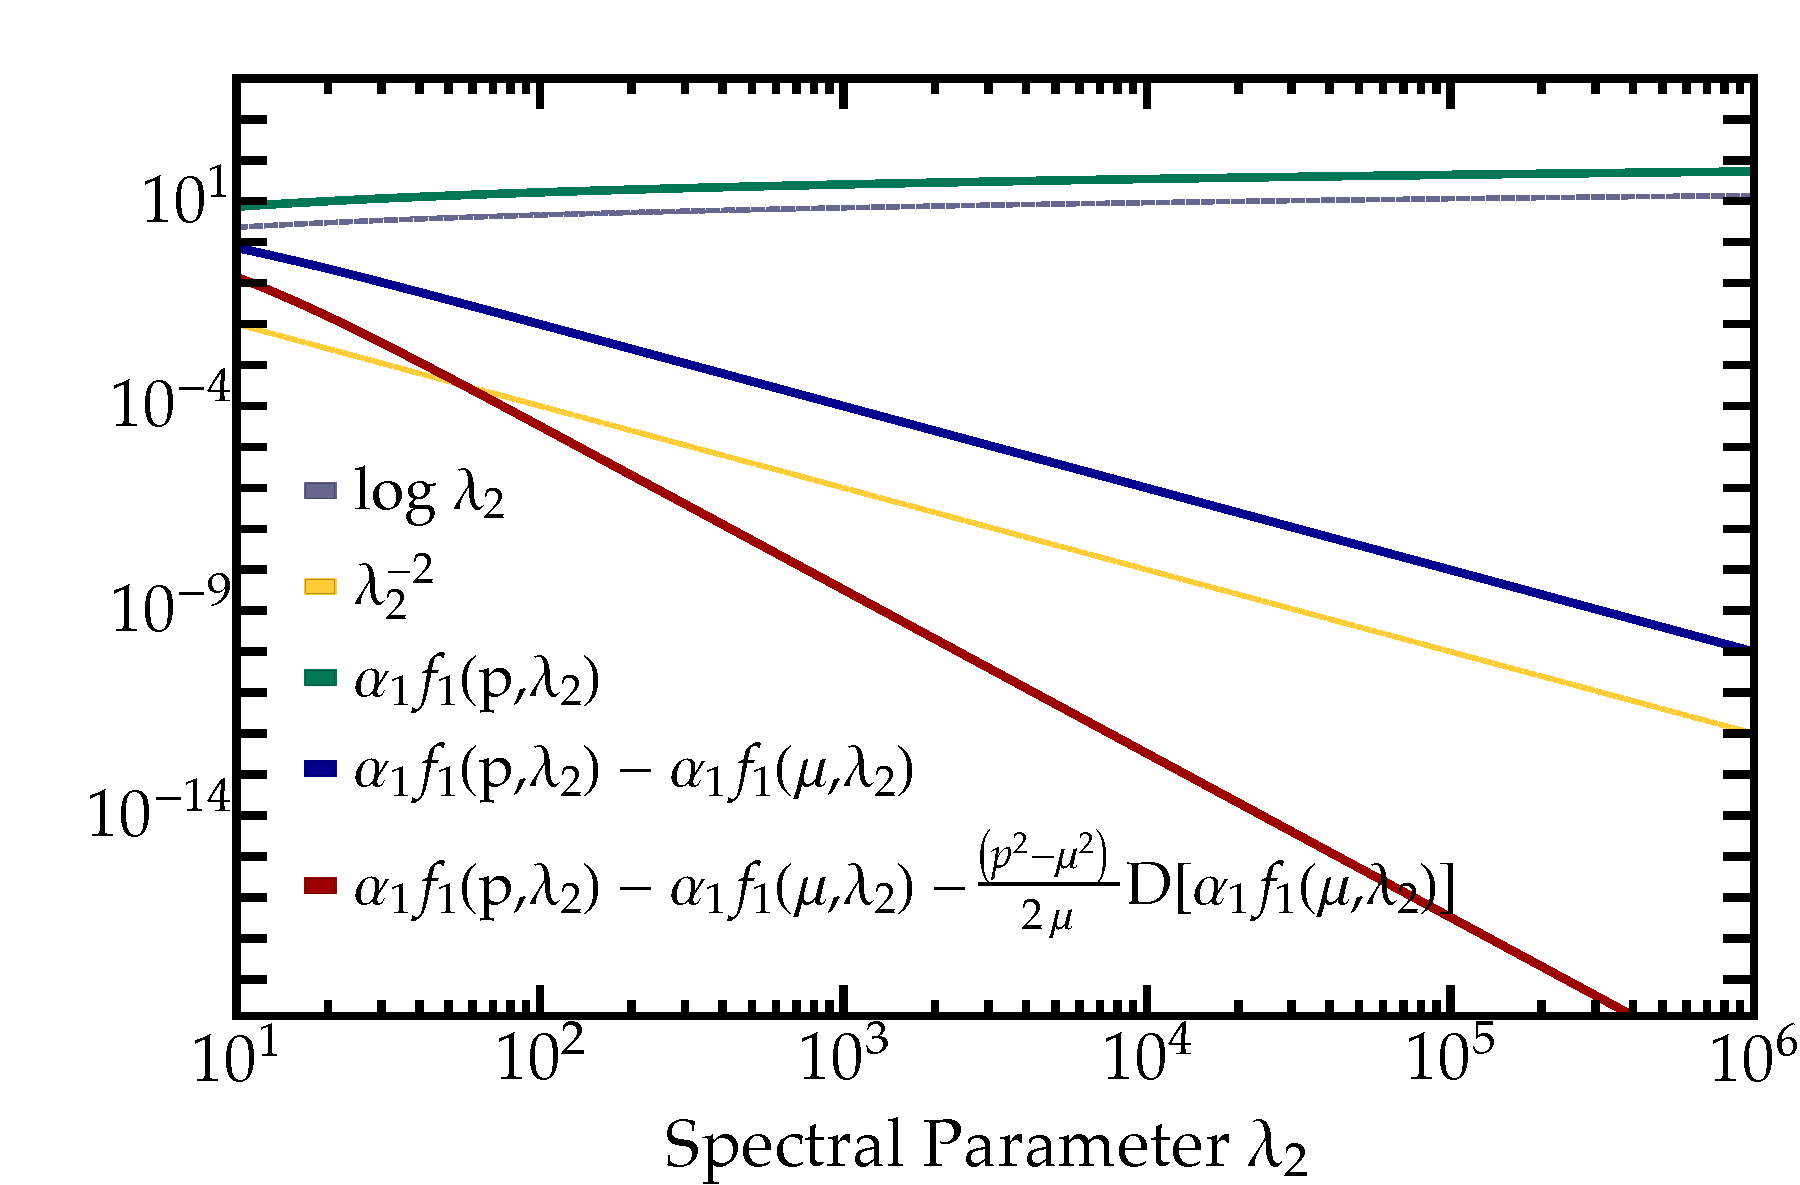
\includegraphics[width = 0.88\textwidth]{figs/plots/FiniteIntegrands1}
	\end{minipage}
	\begin{minipage}{0.8\textwidth}
		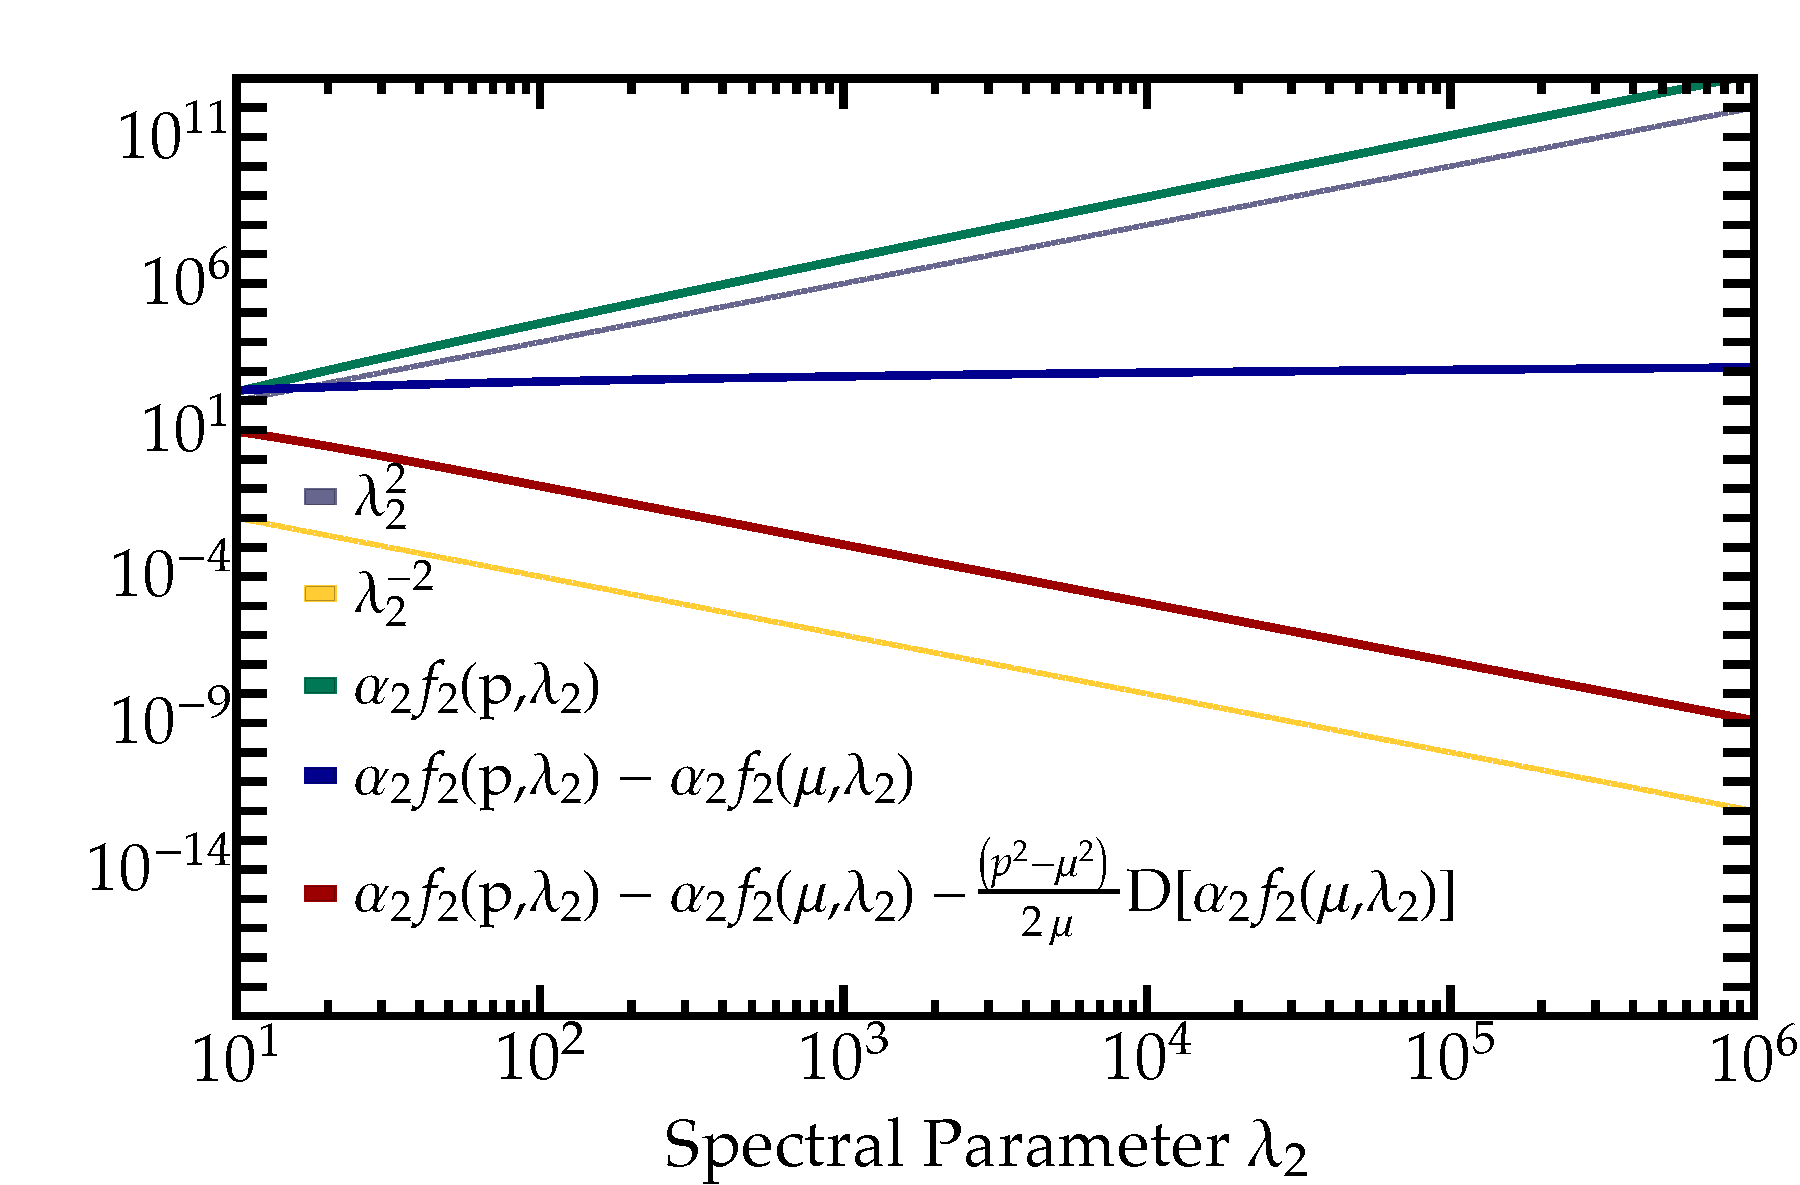
\includegraphics[width = 0.88\textwidth]{figs/plots/FiniteIntegrands2}
	\end{minipage}\caption[Effects of the BPHZ-type subtraction on the integrands, exemplary shown for logarithmically and quadratically divergent parts of the spectral integrand of the Dirac vector part.]{Effects of the BPHZ-type subtraction on the integrands, exemplary shown for logarithmically and quadratically divergent parts of the spectral integrand of the Dirac vector part, cf. \eqref{eqn:IqD}. The other parameters in this plot are fixed to $p=1$ GeV, $\mu = 2$ GeV and $\lambda_1=1$. We checked the effects for various combinations, these specific values were just chosen for demonstration purposes.}
	\label{fig:BPHZ_demonstration}
\end{figure}



\section*{Going to Real Frequencies}
In order to obtain real-time expressions for the computed quantities, we need to evaluate (\ref{eqn:IqD}) and (\ref{eqn:IqM}) at real frequencies, i.\,e. 
\begin{equation}
	I_q^{(D/M)}\left(\omega, \lambda_1, \lambda_2\right) := I_q^{(D/M)}\left(-i(\omega + i0^+)\right).
\end{equation}
 From the definitions of the functions $\alpha_i, \beta_i$ and $\gamma_i$, and $f_i, g_i$ and $h_0$, their respective real-time counterpart is trivially obtained by the substitution $p\leftrightarrow -i\omega$. This is again done in Mathematica, employing the convention $\operatorname{Im}\operatorname{log} x = \pi$\ for $x<0$ for the logarithmic branch cut. 
As a proof of concept, we show that the real-time expression of the Dirac vector part $I_q^{D}\left(\omega\right)$ is in agreement with the expression obtained by explicitly taking the correct limit $\varepsilon\rightarrow 0^+$. We show the real and imaginary parts of  $I_q^{D}\left(-i(\omega + i0^+)\right)$ for different finite values of $\varepsilon$ ranging from $10^{-1}$ to $10^{-5}$ in comparison with the corresponding real-time expression of the diagram $I_q^{D}\left(\omega,\lambda_1,\lambda_2\right)$ in \figref{fig:continuation}.
 \begin{figure}[t] 
\hfill
	\centering
	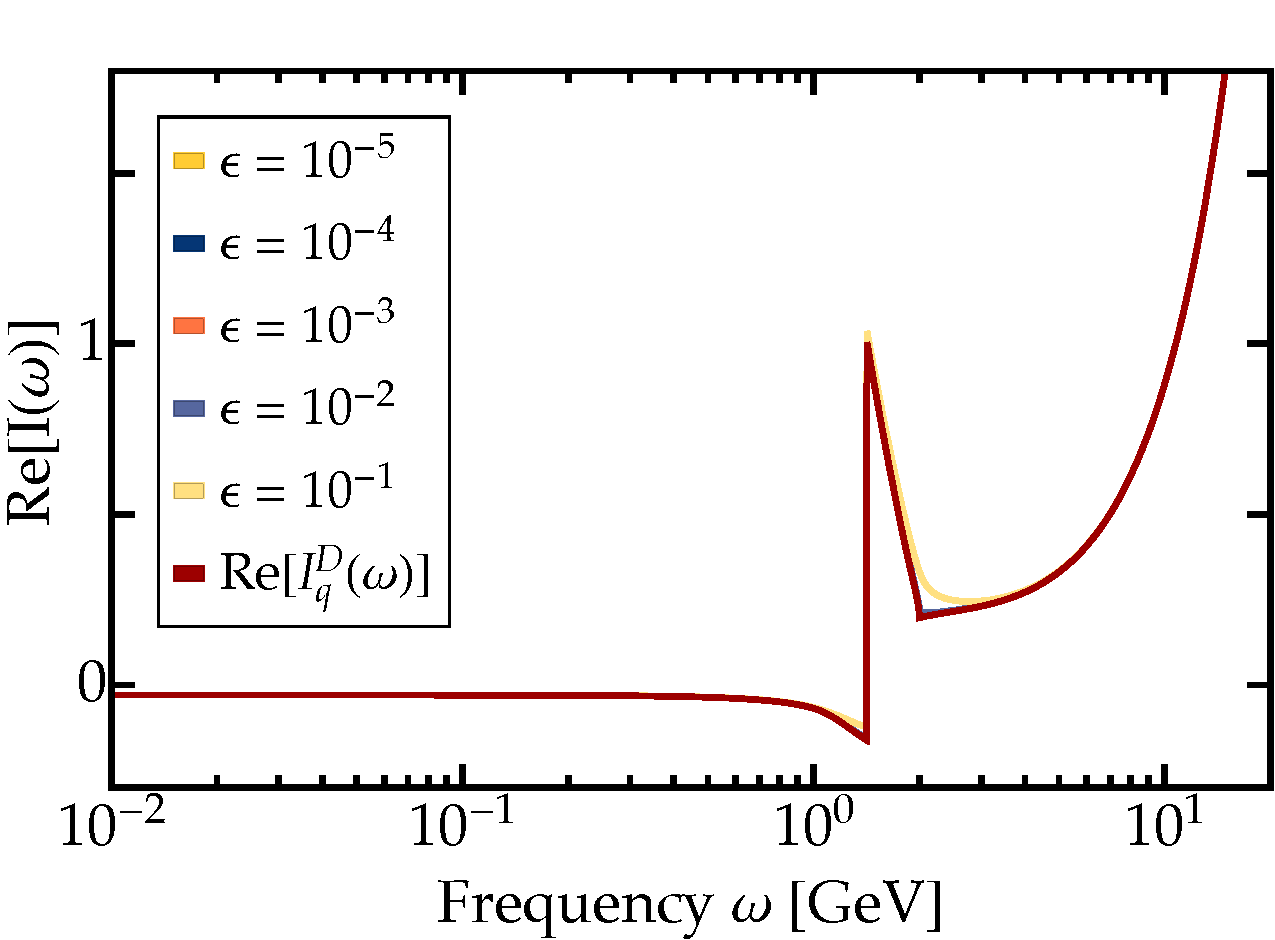
\includegraphics[width = 0.465\textwidth, trim= 4em 0 0 0]{figs/plots/ReContCheck}
\hfill
	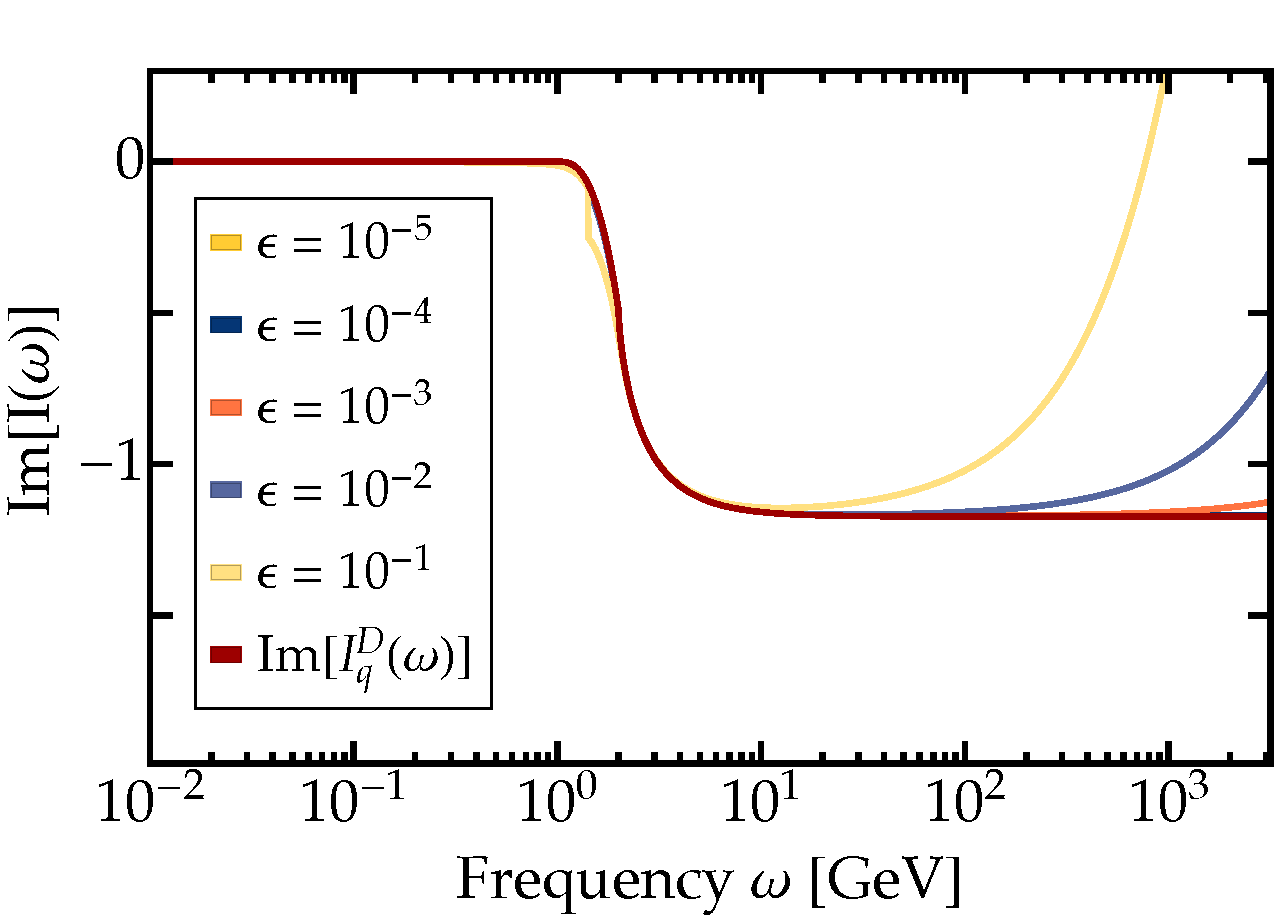
\includegraphics[width = 0.52\textwidth, trim= 0 0.2em 0 0]{figs/plots/ImContCheck}
\hfill
\caption{Real and imaginary parts of the real-time expression $I_q^{D}\left(\omega,\lambda_1,\lambda_2\right)$ in comparison with the correct limit $\varepsilon\rightarrow 0^+$ for different finite values of $\varepsilon$.}
	\label{fig:continuation}
\end{figure}

\section*{Spectral Integrations}
The last step of the calculation consists of performing the (numerical) spectral integrals. With our obtained results for the Euclidean as well as the Minkowski expressions of the regularized integrands at hand, the only missing ingredients are the spectral functions for the gluon and the quarks. In order to be able to perform the spectral integration, appropriate initial \enquote{guesses} for both quark spectral functions $\rho_q^D(\lambda_2)$ and $\rho_q^M(\lambda_2)$ have to be made. In principle, the same would also apply to the gluon spectral function $\rho_A$, but since we have access to an analytic expression for $\rho_A$ from \cite{CyrolPawlowskiRothkopWink2018}, cf. \figref{fig:gluon_specfunc_and_prop}, $\rho_A$ does not need to be updated for every iteration step. For the quarks, we employ quasi-classical spectral functions, reproducing  the classical, perturbative quark propagator
\begin{equation}
	G_q(p) = \frac{-i\slashed{p}+m_q}{p^2+m_q^2}.
\end{equation}
They are simply given by a Dirac delta distribution, rendering the first iteration step trivial. As discussed before, we have to pay attention to the fact, that we are working with a spectral function of a linear argument $\lambda$. We therefore have to be careful with the correct implementation of the Dirac delta distribution. For a composed  function, we know that
\begin{equation}
	(\delta\circ f)(x) = \sum_i^{N_{\mathrm{roots}}}\frac{\delta(x-x_i)}{\abs{f'(x_i)}},
\end{equation}
which implies for our specific case
\begin{equation}
	\delta(x^2-a^2) = \frac{1}{\abs{2a}}\delta(x-a).
\end{equation}
This results in the following expressions for the initially empleyed quark spectral functions:
	\begin{align}
		\rho_{q,\mathrm{init}}^D(\lambda) &= 2\pi i\ \frac{\delta(\lambda-m_q)}{2\lambda}\\
		\rho_{q,\mathrm{init}}^M(\lambda) &= 2\pi m_q\ \frac{\delta(\lambda-m_q)}{2\lambda}.
	\end{align}
This completes our discussion of the calculation of the quark self energy diagram (up to the numerical spectral integrations, that need to be performed in every iteration step for the updated results for the quark spectral functions). Further details on the numerical implementation can be found in \appref{chap:appendixC}.